\documentclass[tikz,border=10pt]{standalone}
\usetikzlibrary{shapes.geometric, arrows.meta, bending}

\definecolor{basepurple}{RGB}{102,43,240}
\definecolor{basered}{RGB}{218,58,50}
\definecolor{basegreen}{RGB}{92,214,41}

\begin{document}
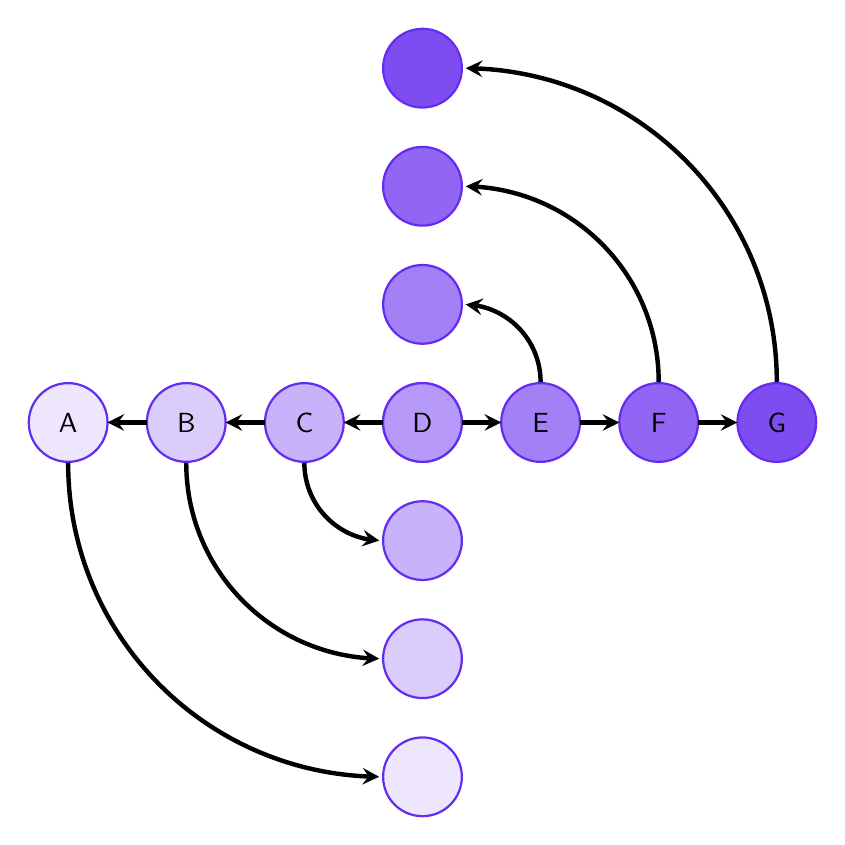
\begin{tikzpicture}[font=\sffamily]
  \tikzset{
    purple_circle/.style args={#1}{
      circle, draw=basepurple, fill=basepurple!#1!white, thick, minimum size=1cm, inner sep=0pt
    },
    arrow_arc/.style={->, >=stealth, ultra thick, shorten >=1pt},
    connecting_arrow/.style={->, >=stealth, ultra thick}
  }

  % Draw the vertical column of circles with different tints of green
  \foreach \x [count=\xi] in {A,...,G} {
    % Define the shade of green based on the current count
    \pgfmathtruncatemacro{\purpleintensity}{\xi * 12}
    \node[purple_circle=\purpleintensity] (V-\x) at (0, 1.5*\xi-6) {};
  }
  
  % Draw the horizontal row of circles with different tints of green
  \foreach \x [count=\xi] in {A,...,G} {
    % Define the shade of green based on the current count
    \pgfmathtruncatemacro{\purpleintensity}{\xi * 12}
    \node[purple_circle=\purpleintensity] (H-\x) at (1.5*\xi-6,0) {\x};

  % Draw arrows in one direction before the fourth node and in the other direction after the fourth node
  \ifnum\xi>4
    \draw[connecting_arrow] (1.5*\xi-7.0,0) -- (1.5*\xi-6.5,0);
  \else
    \ifnum\xi>1
      \draw[connecting_arrow] (1.5*\xi-6.5,0) -- (1.5*\xi-7.0,0);
    \fi
  \fi
  }

% Draw arcs with arrows between he same nodes, skipping the origin
\foreach \x [count=\xi] in {A,...,G} {
  \ifnum\xi=4
  \else
    \draw[arrow_arc, bend right=45] (H-\x) to (V-\x);
  \fi
}

\end{tikzpicture}
\end{document}